\documentclass[../../main.tex]{subfiles}

%-----------------------------------------------------------%
\begin{document}
\section{Mechanical}
\subsection{Loading:}
The satellite is carried to its orbit by a launch vehicle in a flight lasting about 17 minutes.
During this period, the vehicle experiences high levels of acceleration, vibrations and
shocks which are transmitted to the payloads attached to the flight decks of the vehicle.
Launch loads experienced include static loads, vibration loads, acoustic loads and shocks
and impose certain strict requirements on the structure of the satellite. Satellite structure
should be able to withstand these loads during launch. All the components should be
safe and working after the launch. The loading specification for which the launch vehicle
interface is tested is assumed to be the loading data for the satellite during launch. \newline
\newline
    \textbf{Static Loading}

\begin{table}[H]
    \centering
    \begin{tabular}{ |p{3cm} | p{6cm} | p{3cm} | }
    \hline
    \textbf{Direction} & \textbf{Loading} \\
    \hline
    \textbf{Longitudinal} & 3.5g Tensile, 7g Compressive \\
    \hline
    \textbf{Lateral} & 6g Tensile/ Compressive \\
    \hline
    \end{tabular}
    \caption{Static Loads}
    \label{tab:my_label}
\end{table}

\textbf{Harmonic Loading}
\newline
DA-Displacement Amplitude
\begin{table}[H]
    \centering
    \begin{tabular}{ |p{3.5cm}|p{3.5cm}|p{3.3cm}|p{3.3cm}| }
 \hline
     & \textbf{Frequency range(Hz)} & \textbf{Qualification level} &\textbf{Acceptance level} \\
     \hline
\textbf{Longitudinal axis} & (i) 5-8 & 34.5 mm(DA)  & 23 mm (DA) \\
     \hline
 & (ii) 10-100 & 4.5g & 3g \\
 \hline
 \textbf{Lateral axis} & (i) 5-8 & 34.5 mm(DA) & 23 mm(DA) \\
 \hline
 & (ii) 8-100 & 3g & 2g \\
 \hline
\textbf{Sweep rate} & 2 oct/min & 4 oct/min &  \\
 \hline
 \end{tabular}
    \caption{Harmonic Vibration Loads}
    \label{tab:my_label}
\end{table}

\textbf{Random Loading}

\begin{table}[H]
    \centering
    \begin{tabular}{ |p{3cm}|p{3cm}|p{3cm}| }
 \hline
    & \textbf{Qualification} & \textbf{Acceptance} \\
 \hline
\textbf{Frequency(Hz)} &  \textbf{PSD($g^2/Hz$)} &  \textbf{PSD($g^2/Hz$)} \\
\hline
20 & 0.002 & 0.001 \\
\hline
110 & 0.002 & 0.001 \\
\hline
250 & 0.034 & 0.015 \\
\hline
1000 & 0.034 & 0.015 \\
\hline
2000 & 0.009 & 0.004 \\
\hline
g RMS & 6.7 & 4.47 \\
\hline
Duration & 2 min/axis & 1 min/axis \\
\hline
 \end{tabular}
    \caption{Random Vibration Loads}
    \label{tab:my_label}
\end{table}
\subsection{Material Selection:}
\begin{itemize}
    \item Al 6061 T-6 (Structure of Cubesat)- Chosen due to its space heritage. This
material has the best balance of strength to weight ratio, manufacturability
and availability
    \item Mechanical properties of Al 6061 T-6 and other materials used in the satellite
have been tabulated below
\end{itemize}
    \begin{table}[h!]
        \centering
        \begin{tabular}{|p{7cm}|p{2.5cm}|p{2.5cm}|}
             \hline
             \textbf{Properties} & \textbf{AL6061-TS} & \textbf{FR04}\\
             \hline
             \textbf{Density(g/cc)} & 2.7 & 1.85 \\
             \hline
             \textbf{Young’s Modulus(GPa) (X Axis)} & 69 & 20.4 \\
             \hline
             \textbf{Young’s Modulus(GPa) (Y Axis)} & 69 & 18.4 \\
             \hline
             \textbf{Young’s Modulus(GPa) (Z Axis)} & 69 & 15 \\
             \hline
            \textbf{Poisson Ratio(Mpa) (XY Plane)} & 0.33 & 0.11 \\
            \hline
            \textbf{Poisson Ratio(Mpa) (YZ Plane)} & 0.33 & 0.09\\
            \hline
            \textbf{Poisson Ratio(Mpa) (ZX Plane)} & 0.33 & 0.14\\
            \hline
            \textbf{Yield STrength(MPa)} &240 &120\\
            \hline
        \end{tabular}
        \caption{Material Properties}
        \label{tab:my_label}
    \end{table}

    
    \begin{enumerate}
        \item \textbf{Solid Rod and Spacers}
        \begin{table}[h!]
            \centering
            \begin{tabular}{|p{6cm}|p{3cm}|}
                \hline
                \textbf{Component} & \textbf{Material} \\
                \hline
                PCB & FR04 \\
                \hline
                Frame & AL6061-T6 \\
                \hline
                Rods and Spacers & AL6061-T6 \\
                \hline
                Baffle & AL6061-T6 \\
                \hline
            \end{tabular}
            \caption{Material Allocation for Solid Rod CAD}
            \label{tab:my_label}
        \end{table}
        \item \textbf{Support Rails}
        \begin{table}[H]
            \centering
            \begin{tabular}{|p{6cm}|p{3cm}|}
                \hline
                \textbf{Component} & \textbf{Material} \\
                \hline
                PCB & FR04 \\
                \hline
                All Panels & AL6061-T6 \\
                \hline
                Support Rails & AL6061-T6 \\
                \hline
                Baffle, Lens Holder and Optical Image Sensor & AL6061-T6 \\
                \hline    
            \end{tabular}
            \caption{Material Allocation for Support Rails CAD}
            \label{tab:my_label}
        \end{table}
    \end{enumerate}
\subsection {Mesh Generation}
    \begin{enumerate}
        \item \textbf{Mesh Method Features: }
        \begin{itemize}
            \item Multizone meshing was initially used on critical areas like the top panel but it was not continued because it was incompatible with Convergence study feature.
            \item Sweep Meshing was not continued as it could be easily applied on regular/symmetrical components but could not be applied on components like Support Rails.
            \item Only Body Sizing and Automatic Methods were finalized with sizes variable according to part criticality.
        \end{itemize}
        \item \textbf{Mesh Accuracy Features: }Convergence Study was applied on critical components like support rails, Top panel etc. to increase the accuracy of the results but was not continued because of high computation time requirement. Sphere of Influence with radius 5 mm was applied on all screw holes with a mesh refinement of size 1mm inside the region to increase the accuracy of results in critical areas with a limited computation time.
        \begin{figure}[H]
            \centering
            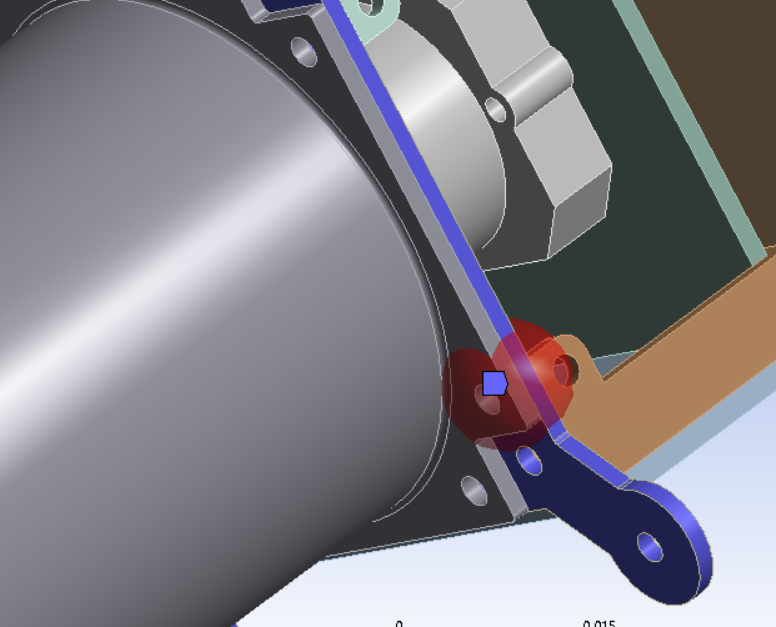
\includegraphics[scale=0.5]{Figures/Mechanical/spoi.PNG}
            \caption{Sphere of Influence-Radius 5mm}
            \label{fig:sys_CAD}
        \end{figure}
    \end{enumerate}
\subsection{Joints \& Contacts }
    \begin{enumerate}
        \item Concentric surfaces were interfaced with the joint to simulate the bond as shown in the figure.
        \item When doing the simulation, fixed joints were used to model screws. All degrees of freedom are constrained in fixed joints. 
      
        \begin{figure}[H]
        \centering
        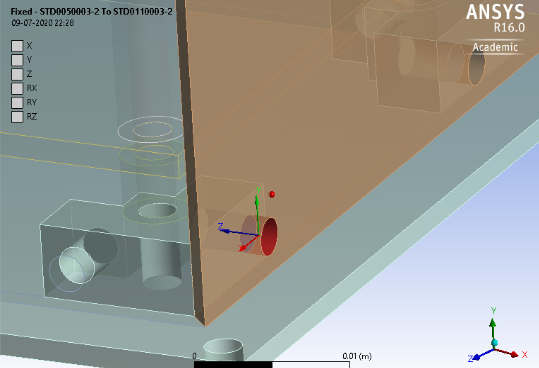
\includegraphics[scale=0.5]{Figures/Mechanical/fixed.png}
        \caption{Fixed Joint}
        \label{fig:sys_CAD}
    \end{figure}
        
        \item Bonded contacts were modelled to simulate adhesives used between two surfaces. They are defined between the rods and the top spacers and also on the interface between the rods and the panels.
        \begin{figure}[H]
        \centering
        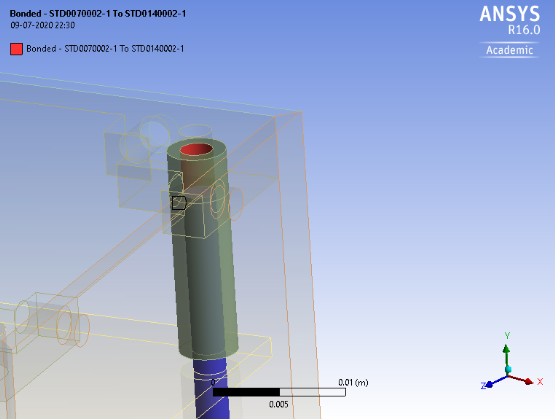
\includegraphics[scale=0.5]{Figures/Mechanical/bonded_contact.png}
        \caption{Bonded Contact}
        \label{fig:sys_CAD}
    \end{figure}
        \item No separation contacts were defined between rods and all the spacers except top ones. No separation contacts will not allow penetration or separation of contact surfaces but allows friction-less sliding in the tangent.
        \begin{figure}[H]
        \centering
        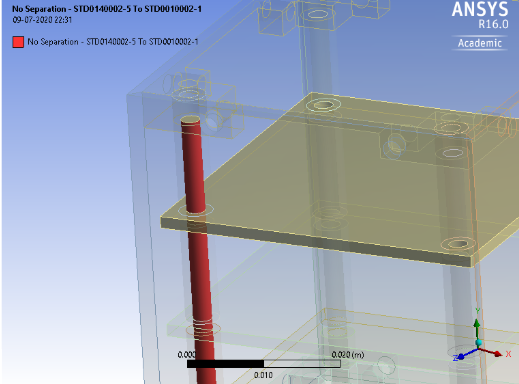
\includegraphics[scale=0.45]{Figures/Mechanical/nosep.png}
        \caption{No-Separation Contact}
        \label{fig:sys_CAD}
    \end{figure}
    \end{enumerate}
\subsection{Simulation Setup and Modelling }
    \begin{enumerate}
        \item \textbf{Solid Rod and Spacers:}
        \begin{enumerate}
            \item \textbf{Model Name:} STD0010002
            \item \textbf{Boundary Conditions:} The CAD was designed targeting the benchmarked Sinclair Interplanetary Star Tracker. It has an extended bottom panel with which it is interfaced with the CubeSats. To model this on Ansys 16.0 we created fixed supports at the outward face of the bottom panel. However, we plan to add a base plate modelling the CubeSats/PS4 and add a fixed support at its face. Further we plan to add fixed joints from the screw holes on the bottom panel corners to the face of the base plate.
            \item \textbf{Mesh Details and Mesh Metrics:}
            \begin{enumerate}
                \item \textbf{Mesh Details: }Automatic meshing was done on all components as the mesh metrics were the best for that type. Spheres of influence with a radius of 2.5mm and an element size of 0.5mm were done on critical parts. 
                \begin{table}[H]
                    \centering
                    \begin{tabular}{|p{3cm}|p{3cm}|}
                    \hline
                    \textbf{Part} & \textbf{Mesh Feature} \\
                    \hline
                    Rods + Spacers & Automatic \\
                    \hline
                    Side Panels & Automatic \\
                    \hline
                    All other components & Automatic \\
                    \hline
                \end{tabular}
                \caption{Meshing Details for Solid Rod CAD}
                \label{tab:my_label}
            \end{table}
                \item \textbf{Mesh Metrics:}
                \begin{table}[H]
                \centering
                \begin{tabular}{|p{3.5cm}|p{3.5cm}|p{3cm}|}
                    \hline
                    \textbf{Property Name} & \textbf{Observed Value(Average)} & \textbf{Ideal Value} \\
                    \hline
                  Element Quality & 0.729 & 1 \\
                  \hline
                  Aspect Ratio & 2.391 & High \\
                  \hline
                  Jacobian Ratio & 1.290 & 1 \\
                  \hline
                  Warping Factor & 4.078E-02 & 0 \\
                  \hline
                Parallel Deviation & 26.40 & - \\

                   \hline
                \end{tabular}
                \caption{Mesh Metrics : Rods \& Spacers Model}
                \label{tab:my_label}
            \end{table}
            \end{enumerate}
            \item \textbf{Joints: } 
            \begin{table}[H]
                \centering
                \begin{tabular}{|p{3cm}|p{3cm}|p{3cm}|}
                    \hline
                    \textbf{Component 1} & \textbf{Component 2} & \textbf{Type of Joint} \\
                    \hline
                   Side Panel & Top Panel & Fixed  \\
                    \hline
                    Side Panel & Bottom Panel & Fixed \\
                    \hline
                    Top Panel & Top Spacer & Fixed \\
                   \hline
                \end{tabular}
                \caption{Joints in Rods \& Spacers Model}
                \label{tab:my_label}
            \end{table}
            \item \textbf{Contacts: }
            \begin{table}[H]
                \centering
                            \begin{tabular}{|p{3cm}|p{5cm}|p{3cm}|}
                    \hline
                    \textbf{Component 1} & \textbf{Component 2} & \textbf{Type of Contact} \\
                    \hline
                   Solid Rod & Bottom Panel& Bonded \\
                    \hline
                    Solid Rod & Top Spacer & Bonded \\
                    \hline
                    Solid Rod & Spacers except top spacer & No separation \\
                    \hline
                    Solid Rod & PCBs & No separation \\
                    \hline
                    Spacers & PCB+Panels & No separation \\
                    \hline

                \end{tabular}
                \caption{Contacts in Rods+Spacers Model}
                \label{tab:my_label}
            \end{table}
            \item \textbf{Results: }
            \begin{enumerate}
            \item \textbf{Static Analysis: Max Equivalent Stress: }
                \begin{table}[H]
                    \centering
                    \begin{tabular}{|p{8cm}|p{6cm}|}
                         \hline
                         \textbf{Component} & \textbf{Max Eq Stress (Pa) \newline(7g Tensile Longitudinal)} \\
                         \hline
                         
                        Solid Rods and Spacers & 7.32E+05 \\
                        \hline
                        Panels & 9.24E+05 \\
                        \hline
                        PCBs  & 3.98E+05 \\
                        \hline
                    \end{tabular}
                    \caption{Static Structural Simulations for Rods+Spacers Model}
                    \label{tab:my_label}
                \end{table}
                \begin{figure}[H]
        \centering
        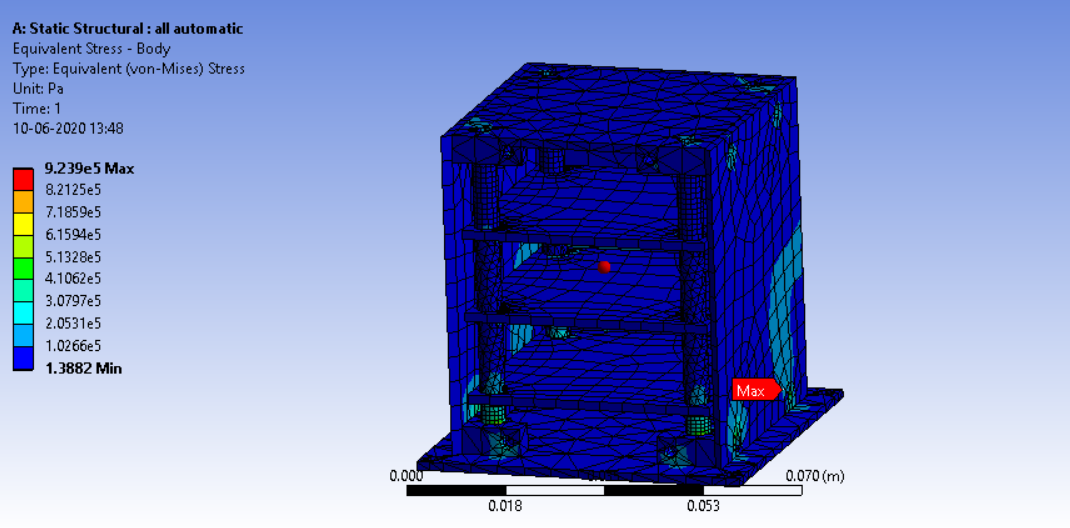
\includegraphics[scale=0.5]{Figures/Mechanical/static.png}
        \caption{Static Simulation : Equivalent Stress}
        \label{fig:sys_CAD}
    \end{figure}
            \item \textbf{Modal Analysis:}
                \begin{itemize}
                    \item Modes Extracted : 300
                    \item First Mode Frequency: 1597.8Hz 
                    \item Max Equivalent Stress: 1.45E+13 \newline
                    \end{itemize}
                    \begin{figure}[H]
        \centering
        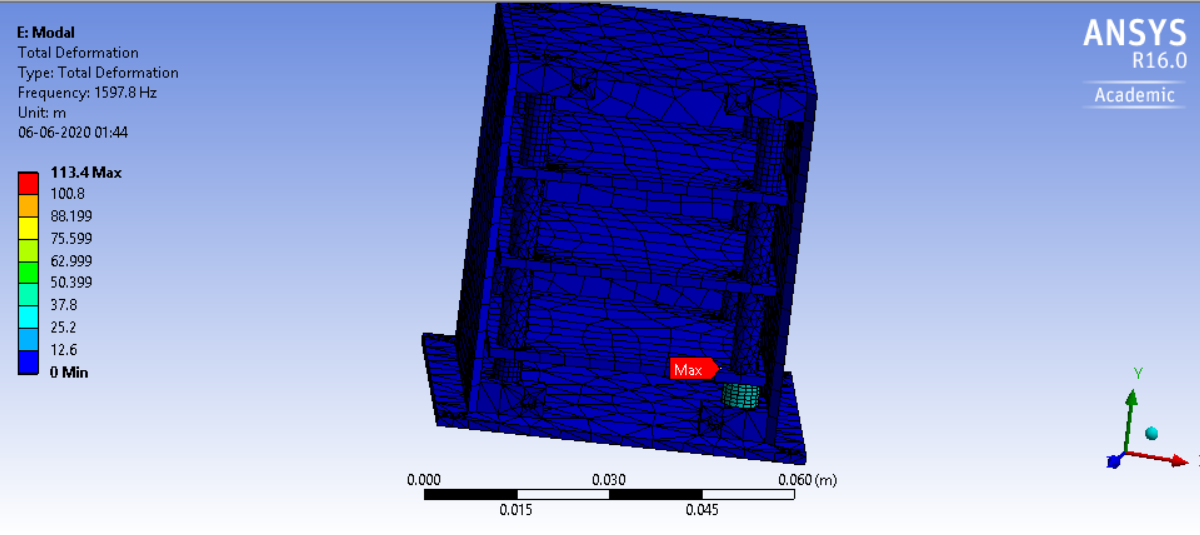
\includegraphics[scale=0.5]{Figures/Mechanical/modal.png}
        \caption{Modal Simulation : Equivalent Stress}
        \label{fig:sys_CAD}
    \end{figure}
            \item \textbf{Harmonic vibration analysis:} Results were recorded for a frequency of 50 Hz.
                \begin{table}[h!]
                    \centering
                    \begin{tabular}{|p{8cm}|p{3cm}|}
                        \hline
                        \textbf{Component} & \textbf{Max Eq Stress (Pa)} \\
                        \hline
                       
                        Solid Rods and Spacers & 4.44E+05 \\
                        \hline
                        Panels & 5.57E+05 \\
                        \hline
                        PCBs  & 2.12E+05 \\
                        \hline
                    \end{tabular}
                    \caption{Harmonic Vibration Analysis Results for Rods+Spacers Model}
                    \label{tab:my_label}
                \end{table}
                \begin{figure}[H]
        \centering
        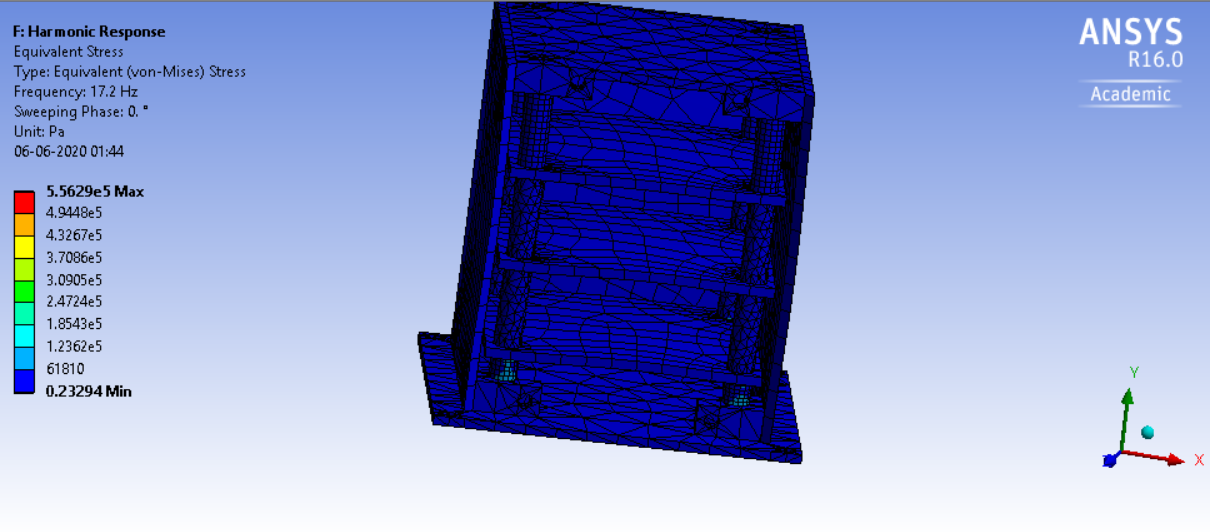
\includegraphics[scale=0.5]{Figures/Mechanical/harmonic.png}
        \caption{Harmonic Simulation : Equivalent Stress}
        \label{fig:sys_CAD}
    \end{figure}
    \newpage
        \item \textbf{Random Vibration Analysis: } Note: Only 100 modes were used and Mode insignificance level was set to 1E-04 to exclude insignificant modes.
                \begin{enumerate}
                    \item \textbf{X Axis: }
                    \begin{table}[h!]
                    \centering
                    \begin{tabular}{|p{8cm}|p{3cm}|}
                        \hline
                        \textbf{Component} & \textbf{Max Eq Stress (Pa)} \\
                        \hline
                       
                        Solid Rods and Spacers & 7.069E+05 \\
                        \hline
                        Panels & 9.199E+05 \\
                        \hline
                        PCBs  & 3.770E+05 \\
                        \hline
                    \end{tabular}
                    \caption{Random Vibrations Analysis for Rods+Spacers Model : X axis}
                    \label{tab:my_label}
                \end{table}
                \begin{figure}[H]
                    \centering
                    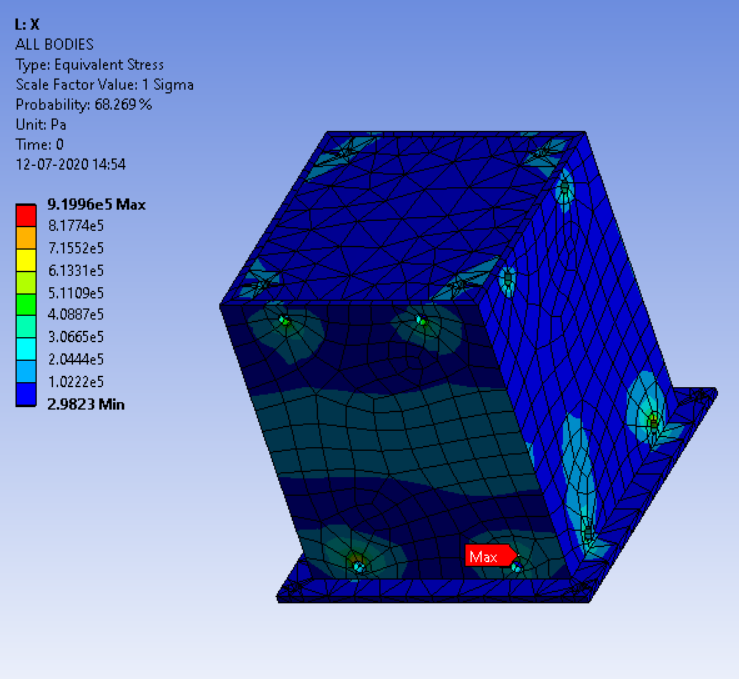
\includegraphics[scale=0.75]{Figures/Mechanical/spacer-rand-X.PNG}
                    \caption{Random Analysis X Axis}
                    \label{fig:sys_CAD}
                \end{figure} 
        \item \textbf{Y Axis: }
                    \begin{table}[h!]
                    \centering
                    \begin{tabular}{|p{8cm}|p{3cm}|}
                        \hline
                        \textbf{Component} & \textbf{Max Eq Stress (Pa)} \\
                        \hline
                     All Solid Rods and Spacers & 1.572E+06 \\
                     \hline
                    All Panels & 3.048E+05 \\
                    \hline
                    All PCBs \& Lens Holder with Optical Image Sensor & 9.441E+05 \\

                        \hline
                    \end{tabular}
                    \caption{Random Vibrations Analysis for Rods+Spacers Model : Y axis}
                    \label{tab:my_label}
                    \end{table}
                    \begin{figure}[H]
                        \centering
                        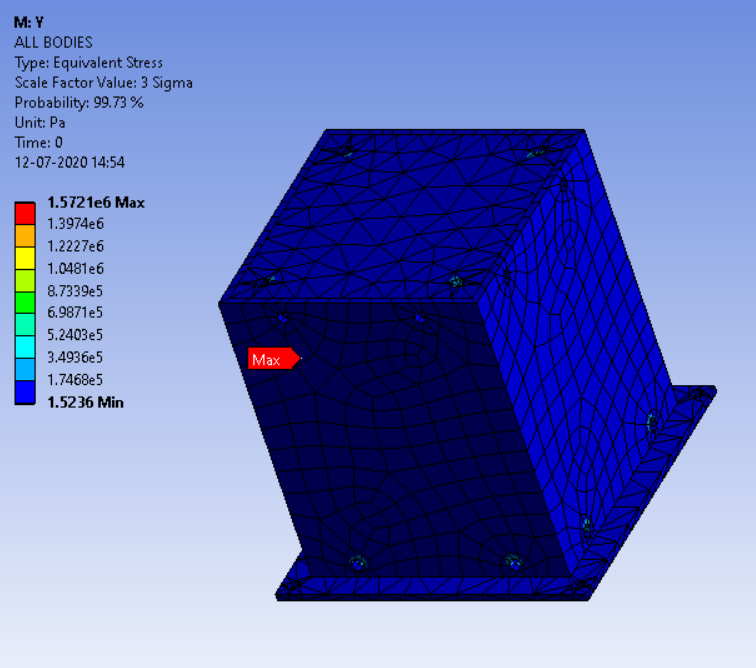
\includegraphics[scale=0.75]{Figures/Mechanical/spacer-rand-Y.PNG}
                        \caption{Random Analysis Y Axis}
                        \label{fig:sys_CAD}
                    \end{figure}
                                \item \textbf{Z Axis: }
                    \begin{table}[h!]
                    \centering
                    \begin{tabular}{|p{8cm}|p{3cm}|}
                        \hline
                        \textbf{Component} & \textbf{Max Eq Stress (Pa)} \\
                        \hline
                     All Solid Rods and Spacers & 7.015E+05 \\
                     \hline
                    All Panels & 9.219E+05 \\
                    \hline
                    All PCBs \& Lens Holder with Optical Image Sensor & 3.174E+05 \\

                        \hline
                    \end{tabular}
                    \caption{Random Vibrations Analysis for Rods+Spacers Model : Z axis}
                    \label{tab:my_label}
                \end{table}
                \begin{figure}[H]
                    \centering
                    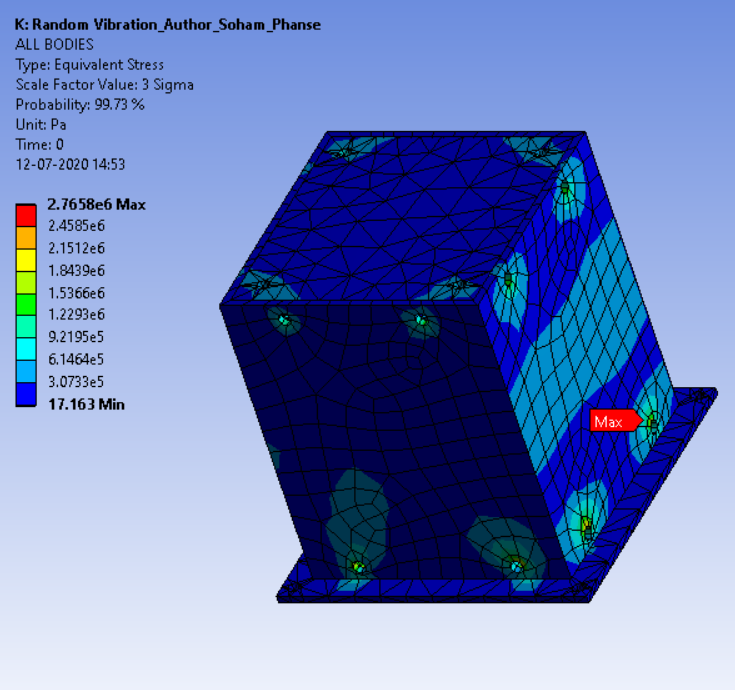
\includegraphics[scale=0.75]{Figures/Mechanical/spacer-rand-Z.PNG}
                    \caption{Random Analysis Z Axis}
                    \label{fig:sys_CAD}
                \end{figure}
                \end{enumerate} 
            \end{enumerate}
        \end{enumerate}
        
        \newpage
        \item \textbf{Support rail:}
        \begin{enumerate}
            \item \textbf{Model Name: }STD0020001\_01
            \item \textbf{Boundary Conditions: }The CAD was designed targeting the benchmarked ST400 Star Tracker. It has four extruded stubs on the top panel for interfacing with the CubeSat. To model this on Ansys 16.0 we created fixed supports at four screw holes on extruded stubs on the top panel.
            \item \textbf{Mesh Details and Mesh Metrics:}
            \begin{enumerate}
                \item \textbf{Mesh Details:} Body Sizing feature was used with a finer mesh in critical areas. A sphere of influence of radius 5mm, centered at geometric centres of all screw holes was created, with a mesh refinement of size 1 mm inside.\newline
                \newline
                \newline
                \begin{figure}[H]
                    \centering
                    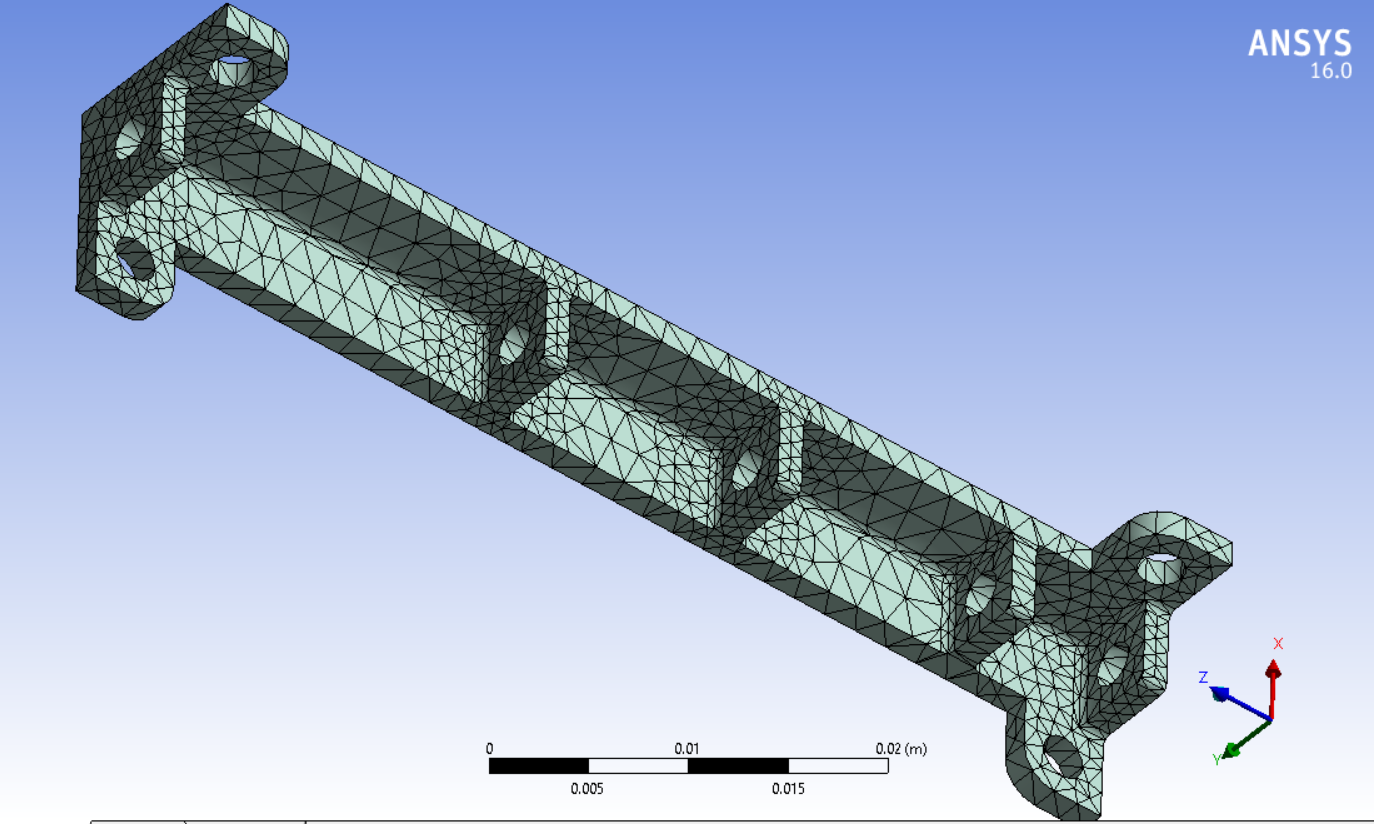
\includegraphics[scale=0.45]{Figures/Mechanical/Support Rail Mesh.PNG}
                    \caption{Mesh - Support Rails}
                    \label{fig:sys_CAD}
                \end{figure}
                \begin{figure}[H]
                    \centering
                    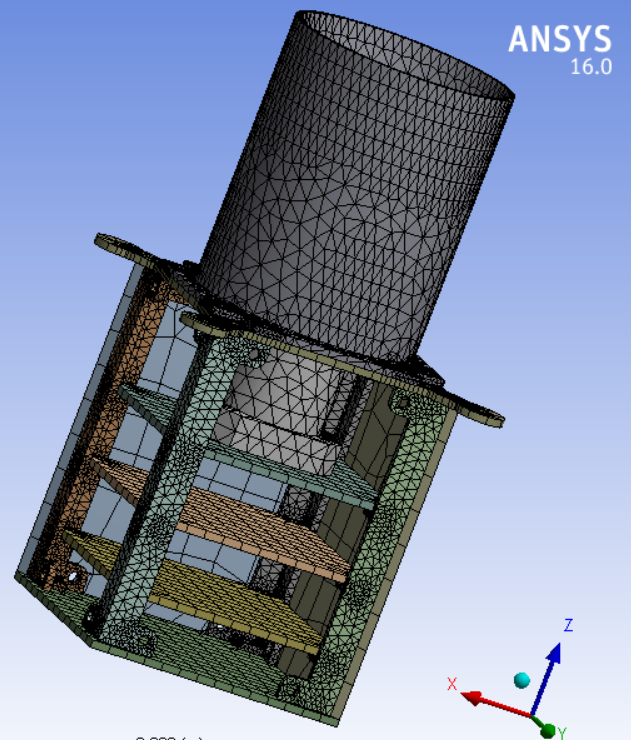
\includegraphics[scale=0.6]{Figures/Mechanical/Entire_STADS_Mesh.PNG}
                    \caption{Mesh - Entire Assembly}
                    \label{fig:sys_CAD}
                \end{figure}
                
                    \begin{table}[h!]
                    \centering
                    \begin{tabular}{|p{5cm}|p{3cm}|p{3cm}|}
                        \hline
                        Part & Mesh Size & Mesh Feature  \\
                        \hline
                        Support Rails & 2 mm & Body Sizing \\
                        \hline
                        Side Panels & 7.5 mm & Body Sizing \\
                        \hline 
                        All other components & 4 mm & Body Sizing \\
                        \hline
                    \end{tabular}
                    \caption{Mesh Details for Support Rails CAD}
                    \label{tab:my_label}
                \end{table}
            \end{enumerate}
            \item \textbf{Joints: }
            \begin{table}[h!]
                \centering
                \begin{tabular}{|p{8cm}|p{3cm}|p{3cm}|}
                    \hline
                    \textbf{Component 1} & \textbf{Component 2} & \textbf{Type of Joint} \\
                    \hline
                    Baffle & Top Panel & Fixed  \\
                    \hline
                    All Panels & Support Rails & Fixed \\
                    \hline
                    All PCBs & Support Rails & Fixed \\
                    \hline
                    Lens Holder and Optical Image Sensor & Optics PCB  & Fixed \\
                    \hline
                \end{tabular}
                \caption{Joints in Support Rails Model}
                \label{tab:my_label}
            \end{table}
            \item \textbf{Contacts:}  No contacts were defined.
            \newline
            \newline
            \newline
            \newline
            \newline
            \newline
            \item \textbf{Results:}
            \begin{enumerate}
                \item \textbf{Static Analysis:} Total Deformation: Entire Assembly: 
                \begin{table}[h!]
                    \centering
                    \begin{tabular}{|p{8cm}|p{6cm}|}
                         \hline
                         \textbf{Component} & \textbf{Max Eq Stress (Pa) \newline(7g Tensile Longitudinal)} \\
                         \hline
                        
                         Support Rails & 6.580E+06 \\
                         \hline
                         All Panels  & 1.693E+07 \\
                         \hline
                         All PCBs \& Lens Holder with Optical Image Sensor & 4.723E+05 \\
                        \hline
                        Baffle & 3.011E+06 \\
                        \hline
                    \end{tabular}
                    \caption{Static Structural Simulations for Support Rails Model}
                    \label{tab:my_label}
                \end{table}
                \begin{figure}[H]
                    \centering
                    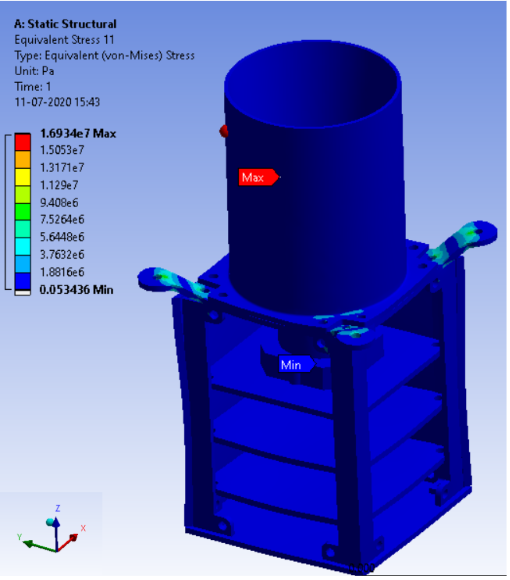
\includegraphics[scale=0.9]{Figures/Mechanical/STATIC.PNG}
                    \caption{ Static Structural Analysis - Entire Assembly }
                    \label{fig:sys_CAD}
                \end{figure}
                \newpage
                \item \textbf{Modal Analysis:}
                \begin{itemize}
                    \item Modes Extracted : 300
                    \item First Mode Frequency: 467.33Hz
                    \begin{table}[h!]
                        \centering
                        \begin{tabular}{|p{3cm}|p{5cm}|}
                            \hline
                            \textbf{Direction} & \textbf{Mass Participation \%} \\
                            \hline
                            X & 0.993953     \\
                            \hline
                            Y & 0.993954     \\
                            \hline
                            Z & 0.994508  \\
                            \hline
                        \end{tabular}
                        \caption{Modal Analysis Results for Support Rail Model}
                        \label{tab:my_label}
                    \end{table}
                    \begin{figure}[H]
                    \centering
                    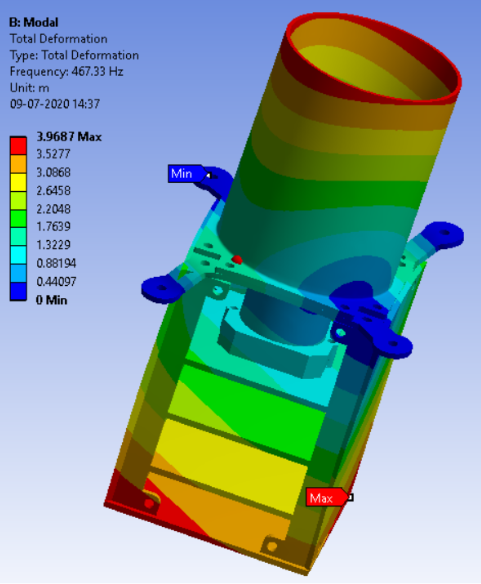
\includegraphics[scale=0.8]{Figures/Mechanical/First_Mode_Shape.PNG}
                    \caption{ First Mode Shape - At 467.33 Hz}
                    \label{fig:sys_CAD}
                \end{figure}
                \end{itemize}
                \newpage
                \item \textbf{Harmonic vibration analysis:} Results were recorded for a frequency of 50 Hz.
                \begin{table}[h!]
                    \centering
                    \begin{tabular}{|p{8cm}|p{3cm}|}
                        \hline
                        \textbf{Component} & \textbf{Max Eq Stress (Pa)} \\
                        \hline
                        
                        Support Rails & 4.097E+06 \\
                        \hline
                        All Panels & 1.018E+07 \\
                        \hline
                        All PCBs \& Lens Holder with Optical Image Sensor & 2.917E+05 \\
                        \hline
                    \end{tabular}
                    \caption{Harmonic Vibration Analysis Results for Support Rails Model}
                    \label{tab:my_label}
                \end{table}
                \begin{figure}[H]
                    \centering
                    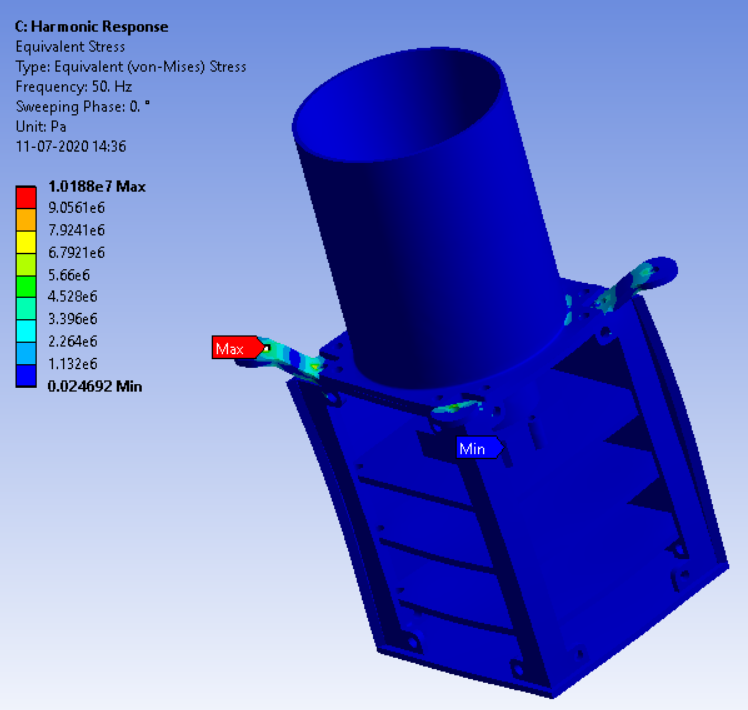
\includegraphics[scale=0.9]{Figures/Mechanical/Harmonic_01.PNG}
                    \caption{ Harmonic Vibration Analysis - Entire Assembly }
                    \label{fig:sys_CAD}
                \end{figure}
                \newpage
                \item \textbf{Random Analysis: }Note: Only 100 modes were used and Mode insignificance level was set to 1E-04 to exclude insignificant modes.
                \begin{itemize}
                    \item \textbf{X - Axis:}
                    \begin{table}[h!]
                        \centering
                        \begin{tabular}{|p{8cm}|p{5cm}|}
                        \hline
                        \textbf{Component} & \textbf{Max Eq Stress (Pa)}\\
                        \hline
                       
                        Support Rails & 3.768E+07 \\
                        \hline
                        All Panels & 4.081E+07 \\
                        \hline
                        All PCBs \& Lens Holder with Optical Image Sensor & 2.106E+06 \\
                        \hline
                        Baffle & 2.941E+07 \\
                        \hline
                        \end{tabular}
                        \caption{Random Analysis for Support Rails Model - X Axis}
                        \label{tab:my_label}
                    \end{table}
                    \begin{figure}[H]
                    \centering
                    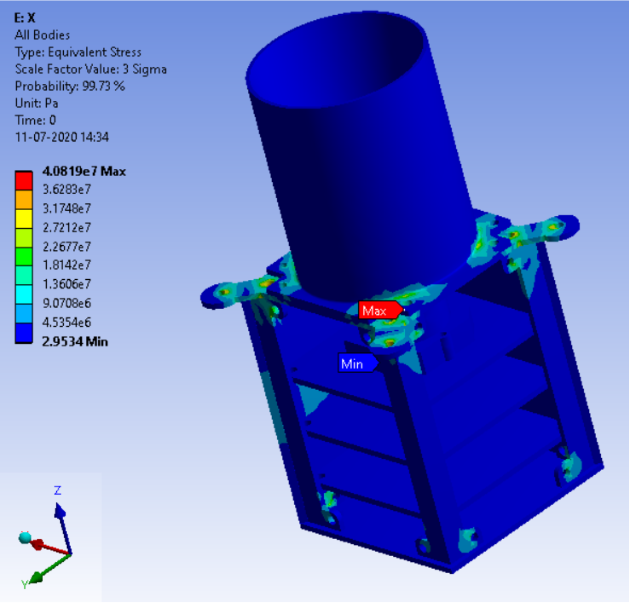
\includegraphics[scale=0.9]{Figures/Mechanical/Random_X.PNG}
                    \caption{ Random Analysis X Axis}
                    \label{fig:sys_CAD}
                    \end{figure}
                    \newpage
                    \item \textbf{Y - Axis:}
                    \begin{table}[h!]
                        \centering
                        \begin{tabular}{|p{8cm}|p{5cm}|}
                        \hline
                        \textbf{Component} & \textbf{Max Eq Stress (Pa)}\\
                        \hline
                        Support Rails & 3.771E+07 \\
                        \hline
                        All Panels & 4.548+07 \\
                        \hline
                        All PCBs \& Lens Holder with Optical Image Sensor & 2.153E+06 \\
                        \hline
                        Baffle & 2.262E+07 \\
                        \hline
                        \end{tabular}
                        \caption{Random Analysis for Support Rails Model - Y Axis}
                        \label{tab:my_label}
                    \end{table}
                    \begin{figure}[H]
                        \centering
                        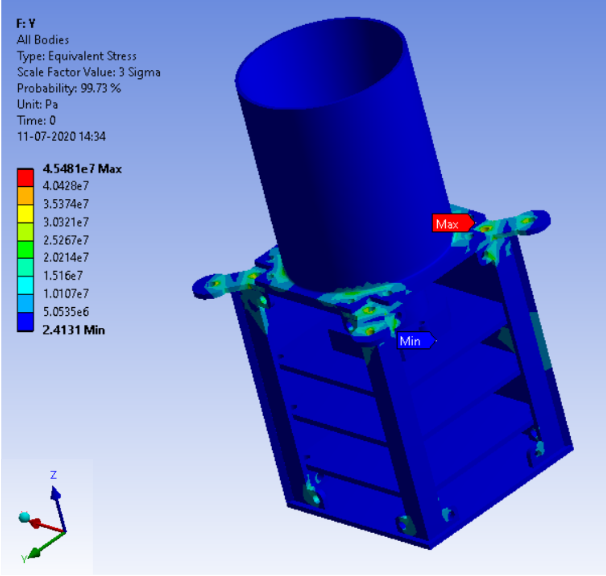
\includegraphics[scale=0.9]{Figures/Mechanical/Random_Y.PNG}
                        \caption{ Random Analysis Y Axis}
                        \label{fig:sys_CAD}
                    \end{figure}
                    \newpage
                    \item \textbf{Z - Axis:}
                    \begin{table}[h!]
                        \centering
                        \begin{tabular}{|p{8cm}|p{5cm}|}
                        \hline
                        \textbf{Component} & \textbf{Max Eq Stress (Pa)}\\
                        \hline
                        
                        Support Rails & 1.052E+08 \\
                        \hline
                        All Panels & 2.175E+08 \\
                        \hline
                        All PCBs \& Lens Holder with Optical Image Sensor & 7.766E+06 \\
                        \hline
                        Baffle & 2.768E+07 \\
                        \hline
                        \end{tabular}
                        \caption{Random Analysis for Support Rails Model - Z Axis}
                        \label{tab:my_label}
                    \end{table}
                    \begin{figure}[H]
                        \centering
                        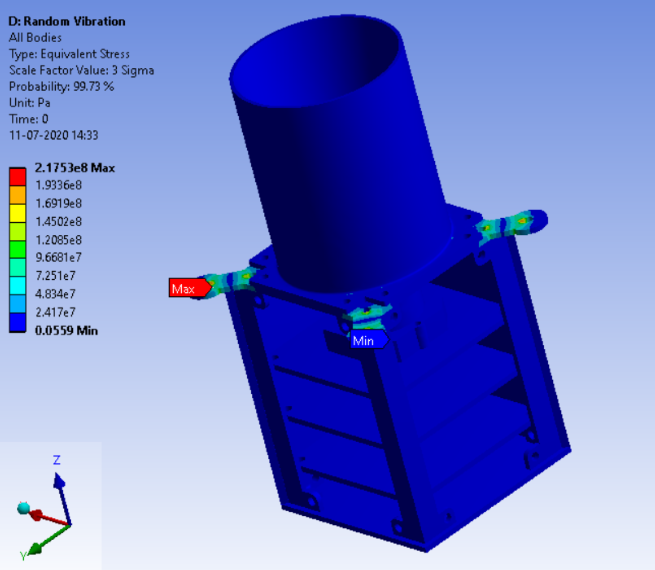
\includegraphics[scale=0.9]{Figures/Mechanical/Random_Z.PNG}
                        \caption{ Random Analysis Z Axis}
                        \label{fig:sys_CAD}
                    \end{figure}
                \end{itemize}
            \end{enumerate} 
        \end{enumerate}
    \end{enumerate}

%----------------------------END----------------------------%
\end{document}